
\de{ĐỀ THI HỌC KỲ I NĂM HỌC 2022-2023}{THPT Tây Thạnh}
\begin{bt}%[0T1B3-5]%[Dự án đề kiểm tra HKI NH22-23- Hieu Phan]%[THPT Tây Thạnh]
Cho hai tập hợp $A=(-\infty ; 3]$ và $B=(-1 ; 4]$. Tìm $A \cap B$, $A \cup B$, $C_{\mathbb{R}} A$, $A\setminus B$.\\
\loigiai{
$A \cap B=\left( -1;3\right]$; $A \cup B=\left( -\infty;4\right]$; $C_{\mathbb{R}} A=\left(3;+\infty\right)$;  $A\setminus B=\left( -\infty;-1\right]$.
}
\end{bt} 

\begin{bt}%[0T3Y1-4]%[Dự án đề kiểm tra HKI NH22-23- Hieu Phan]%[THPT Tây Thạnh]
\immini{
Cho hàm số $y=f(x)$ xác định trên $[-2 ; 6]$ và có đồ thị như hình dưới đây. Tìm các khoảng đồng biến, nghịch biến của hàm số $y=f(x)$.
}{
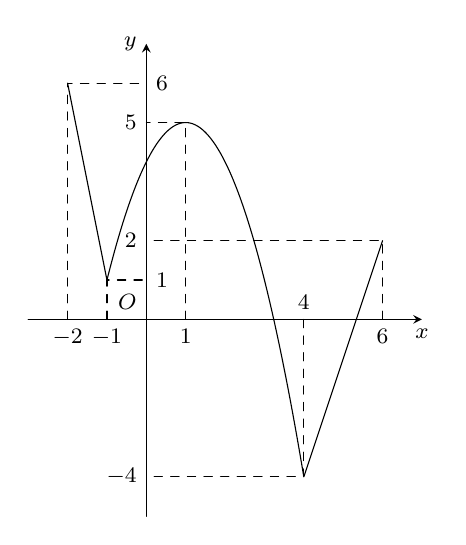
\begin{tikzpicture}[scale=0.5,>=stealth, font=\footnotesize, line join=round, line cap=round]
\def\a{-1} \def\b{2} \def\c{4} % Hệ số
\def\xmin{-3} \def\xmax{7}
\def\ymin{-5} \def\ymax{7}
%\draw[color=gray!50,dashed] (\xmin,\ymin) grid (\xmax,\ymax);
\draw[->] (\xmin,0)--(\xmax,0) node [below]{$x$};
\draw[->] (0,\ymin)--(0,\ymax) node [left]{$y$};
\node at (0,0) [above left]{$O$};
\draw[dashed] (-2,0)node [below]{$-2$}--(-2,6)--(0,6)node [right]{$6$};
\draw[dashed] (-1,0)node [below]{$-1$}--(-1,1)--(0,1)node [right]{$1$};
\draw[dashed] (1,0)node [below]{$1$}--(1,5)--(0,5)node [left]{$5$};
\draw[dashed] (4,0)node [above]{$4$}--(4,-4)--(0,-4)node [left]{$-4$};
\draw[dashed] (6,0)node [below]{$6$}--(6,2)--(0,2)node [left]{$2$};
\draw (4,-4)--(6,2) (-2,6)--(-1,1);
\clip (\xmin+0.1,\ymin+0.1) rectangle (\xmax-0.5,\ymax-0.1);
\draw[smooth,samples=300][domain=-1:4] plot(\x,{\a*(\x)^2+\b*(\x)+\c});
\end{tikzpicture}
}
\loigiai{
Dựa vào đồ thị ta suy ra 
\begin{itemize}
    \item Các khoảng đồng biến là $(-1;1)$, $(4;6)$;
    \item Các khoảng nghịch biến là $(-2;-1)$, $(1;4)$.
\end{itemize} 
}
\end{bt} 

\begin{bt}%[0T3K2-3]%[Dự án đề kiểm tra HKI NH22-23- Hieu Phan]%[THPT Tây Thạnh]
Khảo sát sự biến thiên và vẽ đồ thị $(P)$ của hàm số $y=-x^2+2 x-1$.
\loigiai{
    Tập xác định $ \mathscr{D}=\mathbb{R} $.\\
$y=-x^2+2x-1$ có đỉnh $I(1;0)$.\\
Trục đối xứng $ x=1 $.\\
Bảng biến thiên
\begin{center}
    
\begin{tikzpicture}
        [scale=.8, font=\footnotesize, line join=round, line cap=round, >=stealth]
        \tkzTabInit
        [lgt=2,espcl=3.3] % tùy chọn
        {$x$/1, $y$/2} % cột đầu tiên
        {$-\infty$, $1$, $+\infty$} % hàng 1 cột 2
        \tkzTabVar{-/ $-\infty$, +/ $0$ , -/ $-\infty$} % hàng 3 cột 2
    \end{tikzpicture}
\end{center}
Hàm số nghịch biến trên $ (1; +\infty) $ và đồng biến trên $ (-\infty;1) $.\\
Đồ thị hàm số $y=-x^2+2x-1$\\
\begin{center} 
    % Đồ thị hàm y=ax^2+bx+c. Nếu hệ số lớn cần điều chỉnh hệ trục, vùng lưới, domain và lệnh \clip
    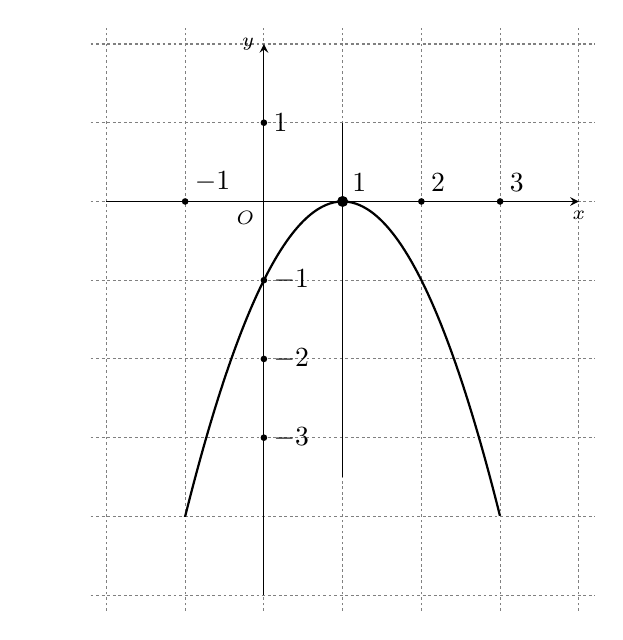
\begin{tikzpicture}[>=stealth,x=1cm,y=1cm,scale=1]
        \def\a{-1} % Hệ số a phải khác 0
        \def\b{2}
        \def\c{-1}
        \draw[color=gray,dash pattern=on 1pt off 1pt,xstep=1.0cm,ystep=1.0cm] (-2.2,-5.2) grid (4.2,2.2);
        \draw[->] (-2,0) -- (4,0) node[below] {\scriptsize $x$};
        \draw[->] (0,-5) -- (0,2) node[left] {\scriptsize $y$};
        \draw (0,0)node[below left]{\scriptsize $O$};
        \draw (1,1) -- (1,-3.5);
        \pgfmathsetmacro\xdinh{-(\b)/2*(\a)}
        \pgfmathsetmacro\ydinh{(4*(\a)*(\c)-(\b)^2)/(4*(\a))}
        \fill[dashed] (\xdinh,\ydinh)circle(2pt) edge (\xdinh,0) edge (0,\ydinh);
        \clip (-3,-4)rectangle(4,2);
        \draw[thick,samples=150,smooth,domain=-4:3] plot(\x,{\a*(\x)^2+(\b)*\x+(\c)});
        \foreach \x in {-1,1,2,3}\fill (\x,0) node[above right]{$ \x $} circle (1.2pt);
        \foreach \y in {-1,1,-2,-3}\fill (0,\y) node[right]{$ \y $} circle (1.2pt);
    \end{tikzpicture}
\end{center} 
}
\end{bt}

 
\begin{bt}%[0T3K2-2]%[Dự án đề kiểm tra HKI NH22-23- Hieu Phan]%[THPT Tây Thạnh]
Xác định parabol $(P)\colon y=a x^2+b x+2 (a \neq 0)$, biết $(P)$ có trục đối xứng $x=\dfrac{3}{2}$ và cắt trục hoành tại điểm $M$ có hoành độ bằng $1$ .
\loigiai{
 Ta có $ (P)\colon \heva{&x=\dfrac{3}{2}  \\ &M(1;0) \in (P)}\Leftrightarrow \heva{& \dfrac{-b}{2a}=\dfrac{3}{2} \\ & 0=a+b+2 }\Leftrightarrow\heva{& 3a+b=0 \\ &a+b=-2 }\Leftrightarrow \heva{& a=1 \\ & b=-3}.$\\
 Vậy    
$(P)\colon y=x^2-3x+2$.
}
\end{bt} 

\begin{bt}%[0T3K2-5]%[Dự án đề kiểm tra HKI NH22-23- Hieu Phan]%[THPT Tây Thạnh]
 Một gia đình sản xuất gạo, do điều kiện nhà xưởng nên mỗi đợt gia đình đó sản xuất được $x \mathrm{~kg}$ gạo. Biết rằng mỗi kg bán được với giá $350-5 x$ (nghìn đồng) và chi phí sản xuất $x \mathrm{~kg}$ gạo là $x^2+5 x+1000$ (nghìn đồng). Hỏi gia đình đó phải sản xuất được bao nhiêu kg gạo để đạt được lợi nhuận tối đa?
\loigiai{
    Chi phí thu được khi sản xuất được $ x $ kg gạo là $ x(350-5x) $.
    Lợi nhuận thu được khi sản xuất $ x $ kg gạo là 
    $$L=x(350-5x)-(x^2+5 x+1000)= -6x^2+345x-1000.$$
    Xét hàm số $ y=-6x^2+345x-1000 $.
    Ta có bảng biến thiên
    \begin{center}
        
\begin{tikzpicture}
            [scale=.8, font=\footnotesize, line join=round, line cap=round, >=stealth]
            \tkzTabInit
            [lgt=2,espcl=3.3] % tùy chọn
            {$x$/1, $y$/2} % cột đầu tiên
            {$-\infty$, $\dfrac{115}{4}$, $+\infty$} % hàng 1 cột 2
            \tkzTabVar{-/ $-\infty$, +/ $\dfrac{31675}{8}$ , -/ $-\infty$} % hàng 3 cột 2
        \end{tikzpicture}
    \end{center}
Dựa vào bảng biến thiên suy ra hàm số đạt giá trị lớn nhất khi $ x= \dfrac{115}{4}=28{,}75$.
Vậy gia đình đó phải sản xuất được $28{,}75$ kg gạo để đạt được lợi nhuận tối đa.
}
\end{bt}

 


\begin{bt}%[0T6B3-1]%[Dự án đề kiểm tra HKI NH22-23- Nguyễn Văn Sơn]%[THPT Tây Thạnh]
	Tìm số trung bình, mốt và tứ phân vị của mẫu số liệu sau đây:
	\begin{center}
		\bf Chiều cao của các thành viên tổ 1 lớp 10C
		\begin{tabular}{|c|c|c|c|c|c|c|c|c|c|}
			\hline
			155 & 165 & 150 & 155 & 165 & 170 & 165 & 150 & 155 & 160 \\
			\hline
		\end{tabular}
	\end{center}
\loigiai{
	\begin{itemize}
	
		\item Số trung bình $\overline{x}=\dfrac{155+165+150+155+165+170+165+150+155+160} {10}=159$
		\item Mốt: $M_{o}=155$ hoặc $M_{o}=165$\\
		Sắp xếp số liệu trên theo thứ tự không giảm, ta được dãy:
			$$150,\ 150,\ 155,\ 155,\ 155,\ 160,\ 165,\ 165,\ 165,\ 170$$
		\item Vì cỡ mẫu là $n=10$ nên tứ phân vị thứ hai là: $Q_2=\dfrac{155+160}{2}=157{,}5$.
		\item Tứ phân vị thứ nhất là trung vị của mẫu: $150,150,155,155,155$. Do đó $Q_1=155$.
		\item Tứ phân vị thứ ba là trung vị của mẫu: $160,165,165,165,170$. Do đó $Q_3=165$.
	\end{itemize}

}
\end{bt}
\begin{bt}%[0T4B2-1]%[Dự án đề kiểm tra HKI NH22-23- Nguyễn Văn Sơn]%[THPT Tây Thạnh]
	Cho tam giác $ABC$ có $BC=10$,$AB=5$, $\widehat{B}=60^\circ$. Tính diện tích và bán kính đường tròn ngoại tiếp tam giác $ABC$.
\loigiai{
	\begin{itemize}
	\item Diện tích $S_{\triangle ABC}=\dfrac{1} {2}BC\cdot AB\cdot \sin B=\dfrac{1}{2} 10\cdot 5\cdot \sin 60^\circ=\dfrac{25\sqrt{3}} {2}$\\
	+ Ta có $AC^2=BC^2+AB^2-2BC\cdot AB\cdot cosB = 10^2+5^2-2\cdot 10\cdot 5\cdot cos60^\circ=75$. Suy ra $AC=\sqrt{75}=5\sqrt{3}$
	\item Bán kính đường tròn ngoại tiếp: $R=\dfrac{AC}{2 \cdot  \sin B}=\dfrac{5\sqrt{3}}{2 \cdot  \sin 60^\circ}=5$
	\end{itemize}
}
\end{bt}
\begin{bt}%[0T9B1-4]%[Dự án đề kiểm tra HKI NH22-23- Nguyễn Văn Sơn]%[THPT Tây Thạnh]
	Cho tam giác $ABC$ có $D$ là điểm đối xứng của $A$ qua $B$ và điểm $M$ thỏa $\vec{BM}=\dfrac{1}{2}\vec{BC}$. Phân tích $\vec{DM}$ theo hai vectơ $\vec{AB}$ và $\vec{AC}$.
\loigiai{
	\hfill
	\begin{center}
	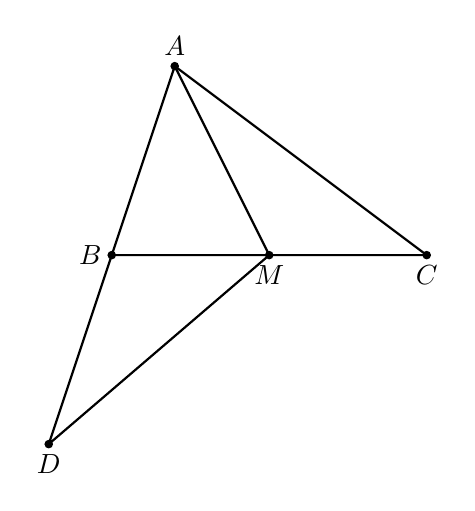
\begin{tikzpicture}[x=1cm,y=1cm,scale=0.8,thick]
		\coordinate (A) at (-1,2) ; 
		\coordinate (B) at (-2,-1) ; 
		\coordinate(D) at (-3, -4);
		\coordinate (C) at (3,-1) ; 
		\coordinate (M) at (0.5,-1) ;
		\draw (A)--(B)--(C)--(A);
		\draw (B)--(D)--(M)--(A) ; 
		\draw[fill] (A) circle (1.4pt) node[above] {$A$};
		\draw[fill] (B) circle (1.4pt) node[left] {$B$};
		\foreach \i in {C,D,M} \draw[fill] (\i) circle (1.4pt) node[below] {$\i$};
	\end{tikzpicture}
	\end{center}
	\begin{itemize}
		\item Giả thiết suy ra $B$ là trung điểm $AD$ và $M$ là trung điểm $BC$. 
		Nên ta có: $\vec{DM}=\vec{AM}-\vec{AD}=\dfrac{1}{2}(\vec{AB}+\vec{AC})-2\vec{AB}=-\dfrac{3}{2}\vec{AB}+\dfrac{1}{2}\vec{AC}$\\
	\end{itemize}
}
\end{bt}
\begin{bt}%[0T5K4-1]%[Dự án đề kiểm tra HKI NH22-23- Nguyễn Văn Sơn]%[THPT Tây Thạnh]
	Cho tam giác $ABC$ có $AB=3, BC=6, AC=8$. Gọi $I$ là điểm trên cạnh $AC$ sao cho $2IA=3IC$. Tính $\vec{CB}$$\cdot\vec{CA}$ và $\vec{BI}$$\cdot\vec{AI}$.
\loigiai{
	\hfill
	\begin{center}
		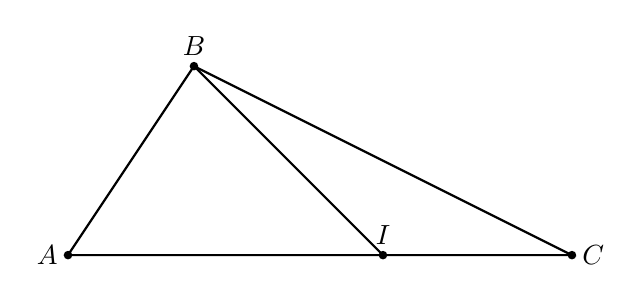
\begin{tikzpicture}[x=1cm,y=1cm,scale=0.8,thick]
			\coordinate (A) at (0,0);
			\coordinate (B) at (2,3);
			\coordinate (C) at (8,0);
			\coordinate (I) at (5,0);
			\draw (A)--(B)--(C)--(A);
			\draw (B)--(I);
			\draw[fill] (A) circle (1.4pt) node[left] {$A$};
			\draw[fill] (B) circle (1.4pt) node[above] {$B$};
			\draw[fill] (C) circle (1.4pt) node[right] {$C$};
			\draw[fill] (I) circle (1.4pt) node[above] {$I$};
		\end{tikzpicture}
	\end{center}
		\begin{itemize}
	\item  Ta có $\cos C=\dfrac{AC^2+CB^2-AB^2}{2\cdot AC\cdot CB}=\dfrac{8^2+6^2-3^2}{2\cdot 8 \cdot 6}=\dfrac{91}{96}$.
	\item  $\vec{CB}$$\cdot\vec{CA} = CB \cdot CA \cdot \cos C=6\cdot 8 \cdot \dfrac{91}{96}=\dfrac{91}{2}$.\\
	Giả thiết suy ra $AI=\dfrac{3}{5} AC = \dfrac{24}{5}$ và $\cos A=\dfrac{AB^2+AC^2-BC^2}{2\cdot AB\cdot AC}=\dfrac{3^2+8^2-6^2}{2\cdot 3 \cdot 8}=\dfrac{37}{48}$\\
	\item $\vec{BI}$$\cdot\vec{AI}=(\vec{AI}-\vec{AB})\cdot\vec{AI}=\vec{AI}^2-\vec{AB} \cdot\vec{AI}=AI^2-AB\cdot AI \cdot \cos A=\left(\dfrac{24}{5}\right)^2-3\cdot\dfrac{24}{5}\cdot \dfrac{37}{48}=\dfrac{597}{50}$.\\
	\end{itemize}
}
\end{bt}
\begin{bt}%[0T5G4-3]%[Dự án đề kiểm tra HKI NH22-23- Nguyễn Văn Sơn]%[THPT Tây Thạnh]
	Cho hình chữ nhật $ABCD$ có $AB=3, AD=4$. Gọi $M$ là điểm thỏa điều kiện $\vec{AM}=k\vec{AB}$. Tìm số thực $k$ để $AC$ vuông góc $DM$.
	\loigiai{
		\hfill
		\begin{center}
		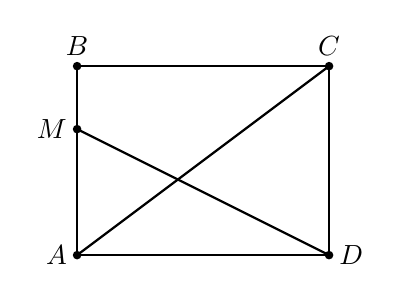
\begin{tikzpicture}[x=1cm,y=1cm,scale=0.8,thick]
			\coordinate (A) at (0,0);
			\coordinate (B) at (0,3);
			\coordinate (C) at (4,3);
			\coordinate (D) at (4,0);
			\coordinate (M) at (0,2);
			\draw (A)--(B)--(C)--(D)--(A);
			\draw (A)--(C);
			\draw (D)--(M);
			\draw[fill] (A) circle (1.4pt) node[left] {$A$};
			\draw[fill] (B) circle (1.4pt) node[above] {$B$};
			\draw[fill] (C) circle (1.4pt) node[above] {$C$};
			\draw[fill] (D) circle (1.4pt) node[right] {$D$};
			\draw[fill] (M) circle (1.4pt) node[left] {$M$};
		\end{tikzpicture}
	\end{center}
	\begin{itemize}
		\item Giả thiết suy ra $AM=kAB=3k$ với $k$ là số dương.\\
		Ta có $\vec{AC} \cdot \vec{DM}$
		$=\left(\vec{AB}+\vec{AD}\right)\cdot\left(\vec{AM}-\vec{AD}\right)$ (Quy tắc hình bình hành và hiệu hai vectơ).\\	$=\vec{AB}\cdot\vec{AM}-\vec{AB}\cdot\vec{AD}+\vec{AD}\cdot\vec{AM}-\vec{AD}^2$\\
		$=AB\cdot AM \cdot \cos 0^\circ - 0 + 0 -4^2$ $=3k^2-16$ (hai vectơ vuông góc có tích vô hướng bằng $0$).\\
		Để $AC$ vuông góc $DM$ thì $\vec{AC} \cdot \vec{DM}=0$. Suy ra $3k^2-16=0$, ta được $k=\dfrac{4\sqrt{3}}{3}$, (vì $k$ là số dương).
	\end{itemize}
	}
\end{bt}